\documentclass[oneside]{article}
\usepackage{fullpage}
\usepackage[pdftex]{graphicx}
\DeclareGraphicsExtensions{.png,.pdf}
\usepackage{hyperref}
\usepackage[format=plain,font=small]{caption}
\usepackage[small]{titlesec}
\usepackage[round,sectionbib]{natbib}
\usepackage{booktabs}
\usepackage[utf8x]{inputenc}

\bibliographystyle{plainnat}
\renewcommand\rmdefault{bch}
\linespread{1.07}

\title{Tidy data}
\author{Hadley Wickham}

\begin{document}
\maketitle

\section{Introduction}

Data cleaning is a vital first step in any analysis, and is often repeated multiple times as new problems come to light. Data cleaning encompasses many activities from outlier checking to missing value imputation. This paper focusses on a small subset of data cleaning that I call data tidying: getting the data in the right format for  manipulation, modelling, and visualisations. This paper defines tidy data, and shows how tidiness makes data easier to work. 

% Other cleaning tasks
%
%  * Parsing dates
%  * Renaming variables
%  * Correcting encoding
%  * Abbreviating long-text strings
%  * Identify how missing values are stored
%  * Strip formatting off numbers and convert to numeric

The principles of tidy data are inspired by databases and Codd's relational algebra, but the set algebra that powers SQL and relational databases is not good a good fit for most statistical problems. It has been driven by my work in data analysis, where I have struggled with many datasets organised in bizarre ways. It grows out of my work on the plyr \citep{me:plyr} and reshape \citep{wickham:2007b} packages in R. These ideas have developed iteratively - as my understanding of tidy data improved, so to did these tools, which made me realise understand better what tools tidy data needs.

My definition of tidy data is not exhaustive, and it focusses on the type of data that statisticians most commonly encounter: rectangular data defined by rows and columns. It is not a good fit for data on networks, \ldots, or \ldots Additional, because the focus of this definition is on explicit definition of the data, it may not be suitable for very large datasets - these may require special infrastructure for performance.

Defining tidy data is important because getting data into the right form for analysis is very important, but there are few existing resources that rigorously define what tidy data is and how to tidy up messy data. A good definition of tidy data also makes messy data easier to work with by showing exactly why it feels dirty and how it can be tidied up. This paper will make life easier for:

\begin{itemize}

\item Applied data scientists, because it will help guide the collection and storage of data.

\item Teachers, by making one part of data cleaning easier to teach by providing a firm theoretical foundation.

\item Data analysts: because you can focus on the problem you are trying to solve, instead of data wrangling.

\end{itemize}

The paper is divided into three sections:

\begin{itemize}

\item Defining tidy data: what are the important characteristics of tidy data, and how can you identify the key components of tidy data from a messy data set.

\item Tidying dirty data: most real world data is not tidy, and in this section what operations are needed to make messy data tidy. These techniques will be illustrated by some of the messy datasets I've encountered in the course of an analysis.

\item Working with tidy data: I'll show how tidy data is easy to model, transform and visualise, and how the tidy data, plus tidy tools, makes previously difficult problems easy. Tidy tools tidy data as input and return tidy data as output, ensuring that data stays tidy throughout the entire analysis.

\end{itemize}

I will illustrate these ideas using R, because that is where I have developed the computational tools to support tidy data, but I believe the principles apply to any programming language which deals with data. In R, the majority built in modelling tools work best with tidy data. The plyr and ggplot2 \citep{me:ggplot2} packages work well with tidy data, and the reshape2 package provides tools useful for making dirty data tidy. The principles of tidy data will also help us criticise existing R functions, and I will show how untidy tools make more work for the analyst.

All code used for cleaning the datasets in this paper is available in the supplemental materials and in the paper repository, \url{https://github.com/hadley/tidy-data}. I'll also provide pointers to other large data tidying and cleaning code sources where appropriate.

Other tools: \citep{kandel:2011}, potter etc.

\section{Defining tidy data}

``Happy families are all alike; every unhappy family is unhappy in its own way.'' ----Leo Tolstoy

Tidy datasets are all alike; every messy dataset is messy in its own way. Here we will define the essence of tidy data, and provide important vocabulary for describing data sets.

Statistical data usually comes in a rectangular \textbf{table}, made up of rows and columns. It is usually labelled with column names, and sometimes with row names. Such data is a collection of \textbf{value}s, each either a single number (if quantitative) or a single string (if qualitative). Values are grouped into \textbf{variables}, measurements of a single attribute. Multiple measurements made on the same \textbf{experimental unit} form an \textbf{observation}. 

Table~\ref{tbl:preg-raw} illustrates a common data format. There are two columns and two rows (plus headers), defining three variables (sex, pregnancy status, count) and four observations.

\begin{table}[htbp]
  \centering
  \begin{tabular}{l|ll}
  \toprule
         & Pregnant & Not-Pregnant \\
  \midrule
  Male   &        0 &            5 \\
  Female &        1 &            4 \\
  \bottomrule
  \end{tabular}
  \caption{Typical data presentation.}
  \label{tbl:preg-raw}
\end{table}

Data is messy or tidy depending on how these structures are arranged. In tidy data each variable lies in a column, and each observation lies in a row. This form is also sometimes called long-form data. We will call all other arrangements messy. An additional restriction is that each table should store data about one type of experimental unit. Table~\ref{tbl:preg-tidy} shows the tidy representation of the previous data.

\begin{table}[htbp]
  \centering
  \begin{tabular}{ll|l}
    \toprule
    pregnant &  sex    & n  \\
    \midrule
    No       &  Female & 4  \\
    No       &  Male   & 5  \\
    Yes      &  Female & 1  \\
    Yes      &  Male   & 0  \\
    \bottomrule
  \end{tabular}
  \caption{Tidied data.}
  \label{tbl:preg-tidy}
\end{table}

While order of variables and observations does not affect analysis, a good ordering makes it easier to scan the raw data. Variables can be ordered by grouping them into identifier and measured variables. \textbf{Identifier variables} describe the experimental design and are known in advance (in a sense they're not really measurements). \textbf{Measured variables} are what we actually measure in the study. Identifier variables should come first first, ordered in terms of their natural hierarchy if present, otherwise alphabetically. Measured variables come next, ordered alphabetically. Rows can then be ordered so that the first id variable varies slowest, followed by the second, and so on.

The following sections describe how to make messy data tidy, and then justify this definition of tidy data by showing how easier it is to work with.

\section{Tidying messy data}

Messy data can be messy in any number of ways, by violating one of the three restrictions, and real data violates these restrictions in almost every way imaginable. In this section, I will focus on some of the most common problems, illustrated with specific datasets:

\begin{itemize}
  \item column headers are values, not variable names
  \item multiple variables are stored in one column
  \item variables are stored in both rows and columns
  \item multiple types of experimental unit stored in the same table
  \item experimental unit stored in the multiple tables
\end{itemize}

The following sections discuss each type of problem in turn, introducing the tools needed to tidy it.

Surprisingly, messy data, including types of messiness not explicitly described above, can be tidied with a surprisingly small set of tools: melting, string splitting, and casting. 

The first step in any tidying is to identify the variables and observations. 

\subsection{Column headers are values, not variables names}

A common case of messy data is tabular data designed for presentation, where variables form both the rows and columns, and column headers are values, not variable names. While I call this type of data messy, in some cases it can be extremely useful. It provides efficient storage for completely crossed designs, and it can provide extremely efficient computation if desired operations can be expressed as matrix operations. It is also necessary for many multivariate methods whose underlying theory is based on manipulation of matrices. But it doesn't generalise well, requiring extensions into higher dimensions to deal with more variables, and can be very inefficient if there are a lot of missing values or variables are nested, not crossed. This makes it inappropriate as a general storage format.

\begin{table}[htbp]
  \centering
  \input{data/pew-raw.tex}
  \caption{Pew survey data on income and religion.} 
  \label{tbl:pew-raw}
\end{table}

Another common use of this format is recording regularly spaced observations over time. For example, the billboard dataset records the date a song first entered the billboard top 100. To record its ranking in the following weeks, 75 variables, from week1 to week75, are needed. This form of storage is useful for data entry because it reduces duplication - otherwise each song in each week would need its own row (a reflection of another messy problem: multiple types of experiment unit stored in the same table).

\begin{table}[htbp]
  \centering
  % latex table generated in R 2.12.0 by xtable 1.5-6 package
% Tue Apr 12 09:10:18 2011
\begin{tabular}{rlllllr}
  \toprule
 year & artist.inverted & track & time & genre & date.entered & week1 \\ 
  \midrule
  2000 & Destiny's Child & Independent Women Part I & 3:38 & Rock & 2000-09-23 &  78 \\ 
  2000 & Santana & Maria, Maria & 4:18 & Rock & 2000-02-12 &  15 \\ 
  2000 & Savage Garden & I Knew I Loved You & 4:07 & Rock & 1999-10-23 &  71 \\ 
  2000 & Janet & Doesn't Really Matter & 4:17 & Rock & 2000-06-17 &  59 \\ 
  2000 & Destiny's Child & Say My Name & 4:31 & Rock & 1999-12-25 &  83 \\ 
  2000 & Iglesias, Enrique & Be With You & 3:36 & Latin & 2000-04-01 &  63 \\ 
  2000 & Sisqo & Incomplete & 3:52 & Rock & 2000-06-24 &  77 \\ 
  2000 & Lonestar & Amazed & 4:25 & Country & 1999-06-05 &  81 \\ 
   \bottomrule
\end{tabular}

  \caption{Billboard top hits for 2000.}
  \label{tbl:billboard-raw}
\end{table}

To tidy up this type of data we need to melt, or stack it, turning columns into rows. Melting is parameterised by a list of variables to keep in columns (cvars), or equivalently a list of columns that should be turned into rows (rvars). It works by adding a new indicator variable to the dataset and stacking the repeated cvars.

\begin{table}[htbp]
  \centering
  \input{data/pew-clean.tex}
  \caption{Pew survey data on income and religion.}
  \label{tbl:pew-clean}
\end{table}

\begin{table}[htbp]
  \centering
  % latex table generated in R 2.12.0 by xtable 1.5-6 package
% Tue Apr 12 09:11:01 2011
\begin{tabular}{rllrlr}
  \toprule
 year & artist & track & week & date & rank \\ 
  \midrule
  2000 & 2 Pac & Baby Don't Cry &   1 & 2000-02-26 &  87 \\ 
  2000 & 2 Pac & Baby Don't Cry &   2 & 2000-03-04 &  82 \\ 
  2000 & 2 Pac & Baby Don't Cry &   3 & 2000-03-11 &  72 \\ 
  2000 & 2 Pac & Baby Don't Cry &   4 & 2000-03-18 &  77 \\ 
  2000 & 2 Pac & Baby Don't Cry &   5 & 2000-03-25 &  87 \\ 
  2000 & 2 Pac & Baby Don't Cry &   6 & 2000-04-01 &  94 \\ 
  2000 & 2 Pac & Baby Don't Cry &   7 & 2000-04-08 &  99 \\ 
  2000 & 2Ge+her & The Hardest Part Of Breaking Up &   1 & 2000-09-02 &  91 \\ 
  2000 & 2Ge+her & The Hardest Part Of Breaking Up &   2 & 2000-09-09 &  87 \\ 
  2000 & 2Ge+her & The Hardest Part Of Breaking Up &   3 & 2000-09-16 &  92 \\ 
  2000 & 3 Doors Down & Kryptonite &   1 & 2000-04-08 &  81 \\ 
  2000 & 3 Doors Down & Kryptonite &   2 & 2000-04-15 &  70 \\ 
  2000 & 3 Doors Down & Kryptonite &   3 & 2000-04-22 &  68 \\ 
  2000 & 3 Doors Down & Kryptonite &   4 & 2000-04-29 &  67 \\ 
  2000 & 3 Doors Down & Kryptonite &   5 & 2000-05-06 &  66 \\ 
   \bottomrule
\end{tabular}

  \caption{Tidied billboard data.}
  \label{tbl:billboard-clean}
\end{table}


\subsection{Multiple variables stored in one column}

After melting, it often happens that the indicator variable actually records information about more than one variable. This is illustrated by the tb dataset - each column represents two values: age and sex.  Table~\ref{tbl:tb-raw} illustrates the raw data. 

\begin{table}[htbp]
  \centering
  % latex table generated in R 2.12.0 by xtable 1.5-6 package
% Mon Apr 11 14:23:26 2011
\begin{tabular}{lrrrrrrrrrr}
  \toprule
 iso2 & year & m04 & m514 & m014 & m1524 & m2534 & m3544 & m4554 & m5564 & m65 \\ 
  \midrule
  AD & 2000 &  &  &   0 &   0 &   1 &   0 &   0 &   0 &   0 \\ 
  AE & 2000 &  &  &   2 &   4 &   4 &   6 &   5 &  12 &  10 \\ 
  AF & 2000 &  &  &  52 & 228 & 183 & 149 & 129 &  94 &  80 \\ 
  AG & 2000 &  &  &   0 &   0 &   0 &   0 &   0 &   0 &   1 \\ 
  AL & 2000 &  &  &   2 &  19 &  21 &  14 &  24 &  19 &  16 \\ 
  AM & 2000 &  &  &   2 & 152 & 130 & 131 &  63 &  26 &  21 \\ 
  AN & 2000 &  &  &   0 &   0 &   1 &   2 &   0 &   0 &   0 \\ 
  AO & 2000 &  &  & 186 & 999 & 1003 & 912 & 482 & 312 & 194 \\ 
  AR & 2000 &  &  &  97 & 278 & 594 & 402 & 419 & 368 & 330 \\ 
  AS & 2000 &  &  &  &  &  &  &   1 &   1 &  \\ 
   \bottomrule
\end{tabular}

  \caption{Original tb data}
  \label{tbl:tb-raw}
\end{table}

Typically, column headers in this format are separated by some character (e.g. {\tt .}, {\tt -}, {\tt \_}, {\tt :}) and we can simply split the string up based on that character. In other cases, such as for this data, more careful string processing is required, or the variable names need to be matched to a hand made table that converts compound values to multiple variables. For the tb data, this yields Table~\ref{tbl:tb-clean}.

\begin{table}[htbp]
  \centering
  \input{data/tb-clean-1.tex}
  \input{data/tb-clean-2.tex}
  \caption{(Left) Molten tb data. (Right) Cleaned data with variable variable broken up in to sex and age variables.}
  \label{tbl:tb-clean}
\end{table}

Storing the data in this form resolves another problem in the original data: it's more informative to compare rates, rather than counts, between countries, but to compute rates we need to know the population in each category. In the original data format, there is no easy way to record this information, and it has to be stored in a separate file. This makes it difficult to correctly match populations to disease counts. In tidy form, adding variables to record total population and disease rate is easier: they just become additional columns.

\subsection{Variables are stored in both rows and columns}

The most complicated form of dirty data is when variables have been stored in both rows and columns. The weather data in Table~\ref{tbl:weather-raw} has variables in single columns (id, year, month), spread across columns (day) and in rows (TMIN, TMAX) (minimum and maximum temperature). Note that the element column is not a variable: it stores the names of variables. Melting the data gets us to Table~\ref{tbl:weather-clean-1}. A useful property of this form of data is that we can drop many of the missing values - they now become implicit rather than explicit. This data is mostly tidy, but we have two variables stored in rows: TMIN and TMAX, the observation type. Fixing this requires the cast, or unstack, operation, which performs the inverse of melting, and rotates the {\tt element} variable back out into the columns to give Table~\ref{tbl:weather-clean-2}. This form has one variable in each column, and each row represents a day's observations. The cast operation is described in more detail in \citet{wickham:2007b}.

\begin{table}[htbp]
  \centering
  % latex table generated in R 2.12.0 by xtable 1.5-6 package
% Mon Apr 11 14:11:47 2011
\begin{tabular}{lrrlrrrrrrrrrr}
  \toprule
 id & year & month & element & d1 & d2 & d3 & d4 & d5 & d6 & d7 & d8 & d9 & d10 \\ 
  \midrule
  MX000017004 & 2010 &   1 & TMAX &  &  &  &  &  &  &  &  &  &  \\ 
  MX000017004 & 2010 &   1 & TMIN &  &  &  &  &  &  &  &  &  &  \\ 
  MX000017004 & 2010 &   2 & TMAX &  & 273 & 241 &  &  &  &  &  &  &  \\ 
  MX000017004 & 2010 &   2 & TMIN &  & 144 & 144 &  &  &  &  &  &  &  \\ 
  MX000017004 & 2010 &   3 & TMAX &  &  &  &  & 321 &  &  &  &  & 345 \\ 
  MX000017004 & 2010 &   3 & TMIN &  &  &  &  & 142 &  &  &  &  & 168 \\ 
  MX000017004 & 2010 &   4 & TMAX &  &  &  &  &  &  &  &  &  &  \\ 
  MX000017004 & 2010 &   4 & TMIN &  &  &  &  &  &  &  &  &  &  \\ 
  MX000017004 & 2010 &   5 & TMAX &  &  &  &  &  &  &  &  &  &  \\ 
  MX000017004 & 2010 &   5 & TMIN &  &  &  &  &  &  &  &  &  &  \\ 
   \bottomrule
\end{tabular}

  \caption{Original weather data}
  \label{tbl:weather-raw}
\end{table}

\begin{table}[htbp]
  \centering
  % latex table generated in R 2.12.0 by xtable 1.5-6 package
% Mon Apr 11 14:09:10 2011
\begin{tabular}{lrrrlr}
  \toprule
 id & year & month & day & element & value \\ 
  \midrule
  MX000017004 & 2010 &   1 &  30 & TMAX & 278 \\ 
  MX000017004 & 2010 &   1 &  30 & TMIN & 145 \\ 
  MX000017004 & 2010 &   2 &   2 & TMAX & 273 \\ 
  MX000017004 & 2010 &   2 &   2 & TMIN & 144 \\ 
  MX000017004 & 2010 &   2 &   3 & TMAX & 241 \\ 
  MX000017004 & 2010 &   2 &   3 & TMIN & 144 \\ 
  MX000017004 & 2010 &   2 &  11 & TMAX & 297 \\ 
  MX000017004 & 2010 &   2 &  11 & TMIN & 134 \\ 
  MX000017004 & 2010 &   2 &  23 & TMAX & 299 \\ 
  MX000017004 & 2010 &   2 &  23 & TMIN & 107 \\ 
   \bottomrule
\end{tabular}

  \caption{Weather data after being melted.}
  \label{tbl:weather-clean-1}
\end{table}

\begin{table}[htbp]
  \centering
  % latex table generated in R 2.12.0 by xtable 1.5-6 package
% Mon Apr 11 14:09:11 2011
\begin{tabular}{lrrrrr}
  \toprule
 id & year & month & day & TMAX & TMIN \\ 
  \midrule
  MX000017004 & 2010 &   1 &  30 & 278 & 145 \\ 
  MX000017004 & 2010 &   2 &   2 & 273 & 144 \\ 
  MX000017004 & 2010 &   2 &   3 & 241 & 144 \\ 
  MX000017004 & 2010 &   2 &  11 & 297 & 134 \\ 
  MX000017004 & 2010 &   2 &  23 & 299 & 107 \\ 
  MX000017004 & 2010 &   3 &   5 & 321 & 142 \\ 
  MX000017004 & 2010 &   3 &  10 & 345 & 168 \\ 
  MX000017004 & 2010 &   3 &  16 & 311 & 176 \\ 
  MX000017004 & 2010 &   4 &  27 & 363 & 167 \\ 
  MX000017004 & 2010 &   5 &  27 & 332 & 182 \\ 
   \bottomrule
\end{tabular}

  \caption{Tidy weather data.}
  \label{tbl:weather-clean-2}
\end{table}

\subsection{Multiple types in one table}

Datasets often involve data collected at multiple levels, on different types of experimental unit. During tidying, each type of experimental unit should be stored in its own table. This makes it easier to spot inconsistencies in the data.

For example, the billboard data describe above actually contains data on two experimental units: the song, and the song-week. These should be broken down into two datasets, a song dataset which stores artist, song name, and a ranking dataset which matches the song and week to the ranking. You could also imagine a week dataset which would record background information about the week, maybe the total number of song sales or similar ``demographic'' information.

% More info about third normal form?

This is closely related to the idea of database normalisation, where each fact is only stored in one location. In Table~\ref{tbl:billboard-clean} you can see facts repeated multiple times: the artist for each track is stored in multiple places. In this case we created the duplication programmatically, so we know that it is consistent, but if the data comes to us in this form we may find inconsistencies. Table~\ref{tbl:billboard-normal} shows the result of normalising the data.

\begin{table}
  \centering
  % latex table generated in R 2.12.0 by xtable 1.5-6 package
% Tue Apr 12 09:43:57 2011
\begin{tabular}{rlll}
  \toprule
 id & artist & track & time \\ 
  \midrule
    1 & 2 Pac & Baby Don't Cry & 4:22 \\ 
    2 & 2Ge+her & The Hardest Part Of Breaking Up & 3:15 \\ 
    3 & 3 Doors Down & Kryptonite & 3:53 \\ 
    4 & 3 Doors Down & Loser & 4:24 \\ 
    5 & 504 Boyz & Wobble Wobble & 3:35 \\ 
    6 & 98° & Give Me Just One Night & 3:24 \\ 
    7 & A*Teens & Dancing Queen & 3:44 \\ 
    8 & Aaliyah & I Don't Wanna & 4:15 \\ 
    9 & Aaliyah & Try Again & 4:03 \\ 
   10 & Adams, Yolanda & Open My Heart & 5:30 \\ 
   11 & Adkins, Trace & More & 3:05 \\ 
   12 & Aguilera, Christina & Come On Over Baby & 3:38 \\ 
   13 & Aguilera, Christina & I Turn To You & 4:00 \\ 
   14 & Aguilera, Christina & What A Girl Wants & 3:18 \\ 
   15 & Alice Deejay & Better Off Alone & 6:50 \\ 
   \bottomrule
\end{tabular}

  \input{data/billboard-rank.tex}

  \caption{Normalised billboard data split up into song and rank datasets.}
  \label{tbl:billboard-normal}
\end{table}

While normalisation is useful for tidying and making sure that there are no inconsistent facts, for analysis it's usually more convenient to denormalise, and collapse back into one giant table: there are few data analysis tools designed to work directly with relational data.

\subsection{One type in multiple tables}

Similarly, it's also common to find data about a single type of experimental unit spread out over multiple tables, or multiple files. These tables are often split up by some other variable, so each file represents a single year, or person, or some other condition. This is typically an easy problem to fix: read in all files, add a new column that records the original file name (because often a variable is stored in the filename), then combine all tables into a single table. This is two or three lines of R code. Once you have a single table, you can perform additional tidying as needed. An example of this type of cleaning can be found at \url{https://github.com/hadley/data-baby-names} which takes 129 yearly baby names tables provided by the US Social Security Administration and combines them into a single file.

A more complicated situation is when the data storage format has changed over time: variable names have changed, different variables have been collected, storage format have changed (e.g.\ csv to tab delimited), or different conventions for missing values have been used. This may require each file to tidied individually (or hopefully in small groups) and then combined together. An example of this type of problem (and solution) can be found at \url{https://github.com/hadley/data-fuel-economy}. That code produces a tidied version of the {\sc epa} fuel economy data. Data from 1978 on is available online, between 1978 and 2008 there have been four major file formats used, with many minor variations.

\section{Working with tidy data}

Tidy data is only worthwhile if it makes analysis easier. This section discusses general tools for working with tidy data, organised into three important components of data analysis: modelling, manipulation and visualisation. These ideas work particularly well together in R, because I have designed the packages to support them, but I will try and focus on the general ideas.

Tidy data is better than messy data because variables are stored in a consistent, and explicit manner, and so tools that work with tidy data have a standard way of referring to variables.  This is a recurring theme for useful analysis tools, whether for modelling, visualisation or data manipulation.

In the absence of tidy data, tools must be much more complicated because they need include some parts of the tidying process. This can be useful for common types of messy data, but typically requires much additional complexity in the function, in both interface and implementation. I also think it's a bad idea because data is so important: you really want to be able to see the results of internal manipulations so that you can verify that they are correct. 

\subsection{Modelling}

Modelling is the inspiration that has driven most of this work, because most modelling tools work best with tidy data. Every statistical language has a way of describing a model as a connection between different variables:   

\begin{itemize}
  \item R (lm): \verb|y ~ a + b + c * d|
  \item SAS (PROC GLM): \verb|y = a + b + c * d|
  \item SPSS (glm): \verb|y BY a b c d |
\end{itemize}

This is not to say that tidy data is the format used internally to compute the regression. Typically significant transformations take place to produce a numeric matrix that can easily be fed to standard linear algebra routines.  Transformations include adding an intercept column (column of all ones), turning categorical variables in to multiple dummy variables, and for smooth terms like splines, projecting the data on to the appropriate basis functions.

There have been some attempts to adapt modelling functions for specific types of messy data. For example in {\sc proc glm} in {\sc sas}, multiple variables on the response side of the equation will be interpreted as repeated measured if the {\sc repeated} keyword is present.  For example, with raw billboard data, you could construct a model of the form \verb|week1-week76 = track| could be used instead of \verb|rank = week * track| on the clean data (provided week is recorded as a categorical variable). \url{http://support.sas.com/documentation/cdl/en/statug/63033/HTML/default/viewer.htm#statug_glm_sect022.htm}.

While model inputs usually require tidy inputs, model outputs, such as predictions and estimated coefficients, aren't always tidy. This makes it more difficult to combine results from multiple models. For example, in R, model coefficients do not have an explicit variable that records the variable name corresponding to an estimate: instead they are recorded as row names.  This is problematic because rownames must be unique, so it's harder to combine coefficients from (e.g.) bootstrap resamples of a model fit.

\subsection{Manipulation}

Data manipulation includes variable-by-variable transformation (e.g. {\tt log} or {\tt sqrt}), as well as aggregation, filtering and reordering.Each operation should be tidy: it should take a tidy input and return a tidy output - if so I call it a tidy tool. Tidy tools are important because they are composable: you can chain them together without having to worry about changing data formats.

In my experience there are four extremely common operations that are performed over and over again in the course of an analysis. These are the four fundamental verbs of data manipulation:

\begin{itemize}

\item filtering, or subsetting, where some observations are removed
\item aggregation, where multiple values are collapsed into a single value
\item reordering, where the order of observations is changed
\item mutation, where new variables are added or existing variables modified 

\end{itemize}

These four verbs can be, and often are, modified by the \textbf{by} preposition. Many times we need group-wise aggregates, transformations or subsets: pick the biggest in each group, average over replicates, ... Some aggregations occur so frequently they deserve their own optimised implementations. An example of one such operation is (weighted) counting. Base R provides the {\tt table} function for this, but it is not tidy: it returns a a messy multidimensional table. An tidy alternative is the {\tt count} function from plyr.

These tools are most useful when they are tidy, and this distinction provides a useful tool for critiquing built in R data analysis tools. {\tt subset}, {\tt transform}, and {\tt aggregate} are tidy. {\tt by}, {\tt xtabs} and {\tt tapply} are not. Not being tidy doesn't mean a tool isn't useful, it just makes it hard to string together during data analysis - which slows down analysis, because you have remember how to tidy that particular format.

Other tools are need for dealing with multiple datasets.  

\begin{itemize}

\item {\tt join}: An advantage of long form data is the ease with which it can be combined: we just need a join operator which works by matching common variables and adding new columns. Compare this to the difficulty of combining wide datasets stored in arrays - these typically require painstaking alignment before matrix operations can be used, and errors are very hard to detect. 

\item {\tt match\_df}: Another common operation is subsetting individual level data based on some summary level statistic. This is accomplished using a function very similar to join that only returns matching rows instead of trying to combine the columns.

\end{itemize}

% Need a comparison of tidy data vs. multi-d array.
% Things that are easy with arrays: sweep, apply, prop.table
% Things that are hard with arrays: merge, lm

\subsection{Visualisation}

Tidy data works well with visualisation because it connects closely to the grammar of graphics \citep{wilkinson:2006}. With tidy data, visualisations are straightforward to describe as a mapping between variables and aesthetic properties like position, size, shape and colour. This is the idea behind the layered grammar of graphics \citep{wickham:2007d}, as implemented in the ggplot2 package in R.

Something about the group aesthetic - how this makes certain types of graphics much easier.

This type of data is so common that in R a number of graphical tools have been designed specifically to visualise it, e.g. {\tt barplot}, {\tt matplot}, {\tt dotchart}, {\tt mosaicplot}. Other tools are designed to provide common manipulations like {\tt sweep}, {\tt prop.table} and {\tt margin.table}. Other tools produce this data format from formerly tidy data: {\tt table}, {\tt xtabs}, {\tt tapply}.

\section{Case study} 

The following case study attempts to illustrate how tidy data makes a data analysis easier, combining manipulation, visualisation and modelling. The case study uses data on mortality in Mexico, with the goal of finding diseases that have notably different rates from the average over the course of the day. The original data and cleaning code can be found at \url{https://github.com/hadley/mexico-mortality}. It illustrates some of the many challenges apart from tidying that data cleaning requires: getting variables into the right formats, removing clearly impossible values, and finding good sources of data.

We start by aggregating the full dataset to the minimal data that will allow us to answer our question: the number of deaths per hour per disease:

\begin{verbatim}
# Counting the the number of deaths in each hour of the day for each 
# cause of death
hod2 <- count(deaths, c("hod", "cod"))

# Removing missing missing observations
hod2 <- subset(hod2, !is.na(hod))

# Combine with data set that gives disease names
hod2 <- join(hod2, codes)

# Convert from counts to proportions within each disease
hod2 <- ddply(hod2, "cod", transform, prop = freq / sum(freq))
\end{verbatim}

Next, we compute the overall average death rate for each hour, and merge that back to the original data.

\begin{verbatim}
overall <- ddply(hod2, "hod", summarise, freq_all = sum(freq))
overall <- mutate(overall, prop_all = freq_all / sum(freq_all))

hod2 <- join(overall, hod2, by = "hod")
\end{verbatim}

\begin{table}
  \centering
  % latex table generated in R 2.12.0 by xtable 1.5-6 package
% Wed Apr 20 08:16:24 2011
\begin{tabular}{rllrrrr}
  \toprule
 hod & cod & disease & freq & prop & freq\_all & prop\_all \\ 
  \midrule
    1 & A01 & Typhoid and paratyphoid fevers &   3 & 0.06 & 20430 & 0.04 \\ 
    1 & A02 & Other salmonella infections &   3 & 0.05 & 20430 & 0.04 \\ 
    1 & A04 & Other bacterial intestinal infections &   7 & 0.05 & 20430 & 0.04 \\ 
    1 & A05 & Other bacterial foodborne intoxications, not... &   1 & 0.05 & 20430 & 0.04 \\ 
    1 & A06 & Amebiasis &   2 & 0.02 & 20430 & 0.04 \\ 
    1 & A09 & Diarrhea and gastroenteritis of infectious... & 112 & 0.04 & 20430 & 0.04 \\ 
    1 & A15 & NA &   2 & 0.01 & 20430 & 0.04 \\ 
    1 & A16 & Respiratory tuberculosis, not confirmed... &  53 & 0.03 & 20430 & 0.04 \\ 
    1 & A17 & Tuberculosis of nervous system &   2 & 0.02 & 20430 & 0.04 \\ 
    1 & A18 & Tuberculosis of other organs &   5 & 0.05 & 20430 & 0.04 \\ 
    1 & A19 & Miliary tuberculosis &   8 & 0.05 & 20430 & 0.04 \\ 
    1 & A37 & Whooping cough &   1 & 0.10 & 20430 & 0.04 \\ 
    1 & A41 & Other septicemia & 180 & 0.04 & 20430 & 0.04 \\ 
    1 & A46 & Erysipelas &   1 & 0.04 & 20430 & 0.04 \\ 
    1 & A48 & Other bacterial diseases, not elsewhere... &   1 & 0.07 & 20430 & 0.04 \\ 
   \bottomrule
\end{tabular}

  \caption{First fifteen rows of the {\tt hod2} data frame.}
  \label{tbl:counts}
\end{table}

Next we compute a measure of deviation between each disease and the overall trend: a mean squared deviation. We don't know the variance characteristics of this estimator, so we explore it empirically in Figure~\ref{fig:deviation} by plotting n vs\. deviation. On the log-log scale there is a clear linear trend and inspecting the coefficient of linear model indicates that error is proportional $1 / n^0.9$. We are interested in the outliers who have relatively high values relative to the variability: these are diseases which are different from the average.

\begin{figure}[htbp]
  \centering
  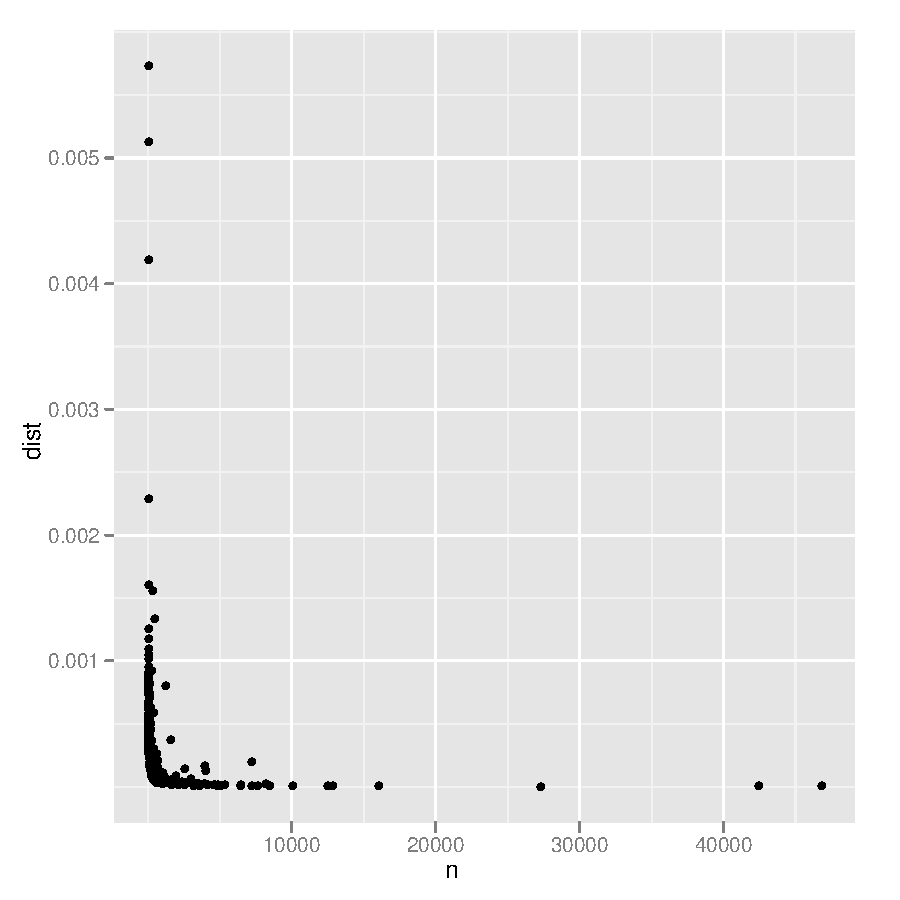
\includegraphics[width=0.5\linewidth]{case-study/n-dist-raw.pdf}%
  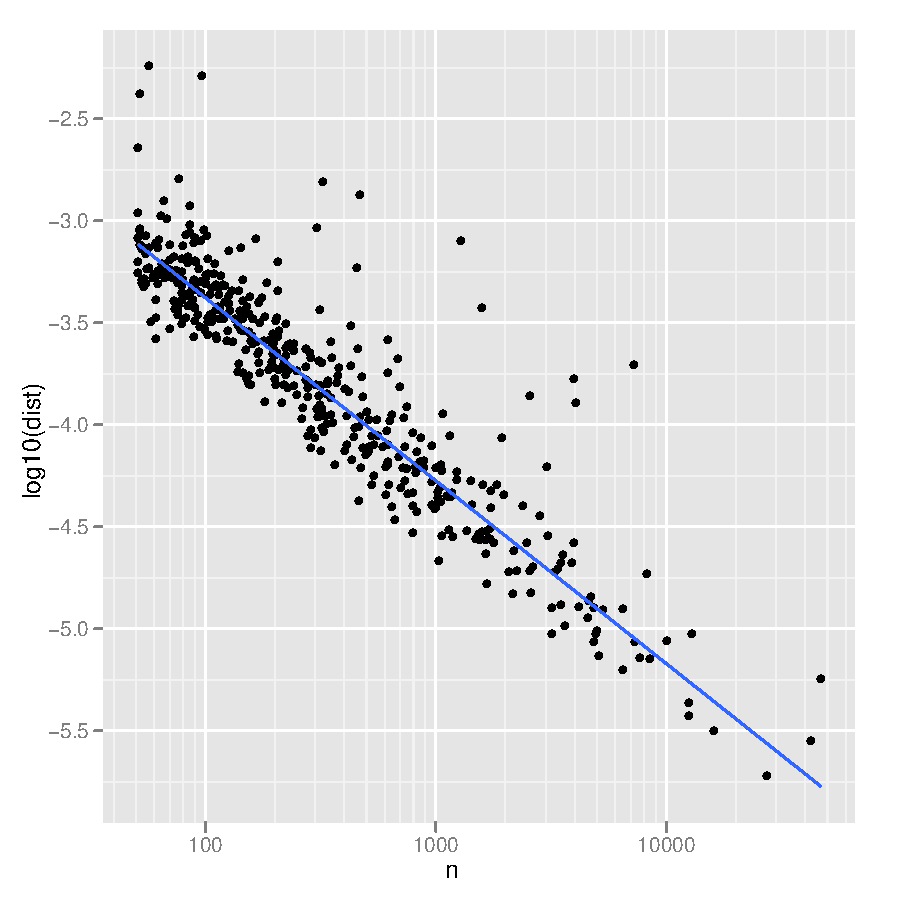
\includegraphics[width=0.5\linewidth]{case-study/n-dist-log.pdf}
  \caption{(Left) Plot of n vs deviation. Variability of deviation dominated by the sample size: small samples have large variability. (Right) Log-log plot makes it easy to see pattern of variation as well as unusually high values.  Overlaid with robust linear fit.}
  \label{fig:deviation}
\end{figure}

\begin{verbatim}
devi <- ddply(hod2, "cod", summarise, n = sum(freq), 
  dist = mean((prop - prop_all)^2))
devi <- subset(devi, n > 50)
\end{verbatim}

A plot (not shown) of n vs\. the residuals shows the break around 1.5, so we select those diseases and plot their time courses in two plots. We break the diseases into two groups because of the differences in variability. The results are shown in Figure~\ref{fig:disease}. The causes of death fall in to three main groups: homicide, drowning, transportation and electrical. Murders are more common at night, drowning in the afternoon, traffic during commute times, and drowning in the afternoon. The only disease is sudden infant death syndrome, which has a large peak in early morning.

\begin{figure}[htbp]
  \centering
    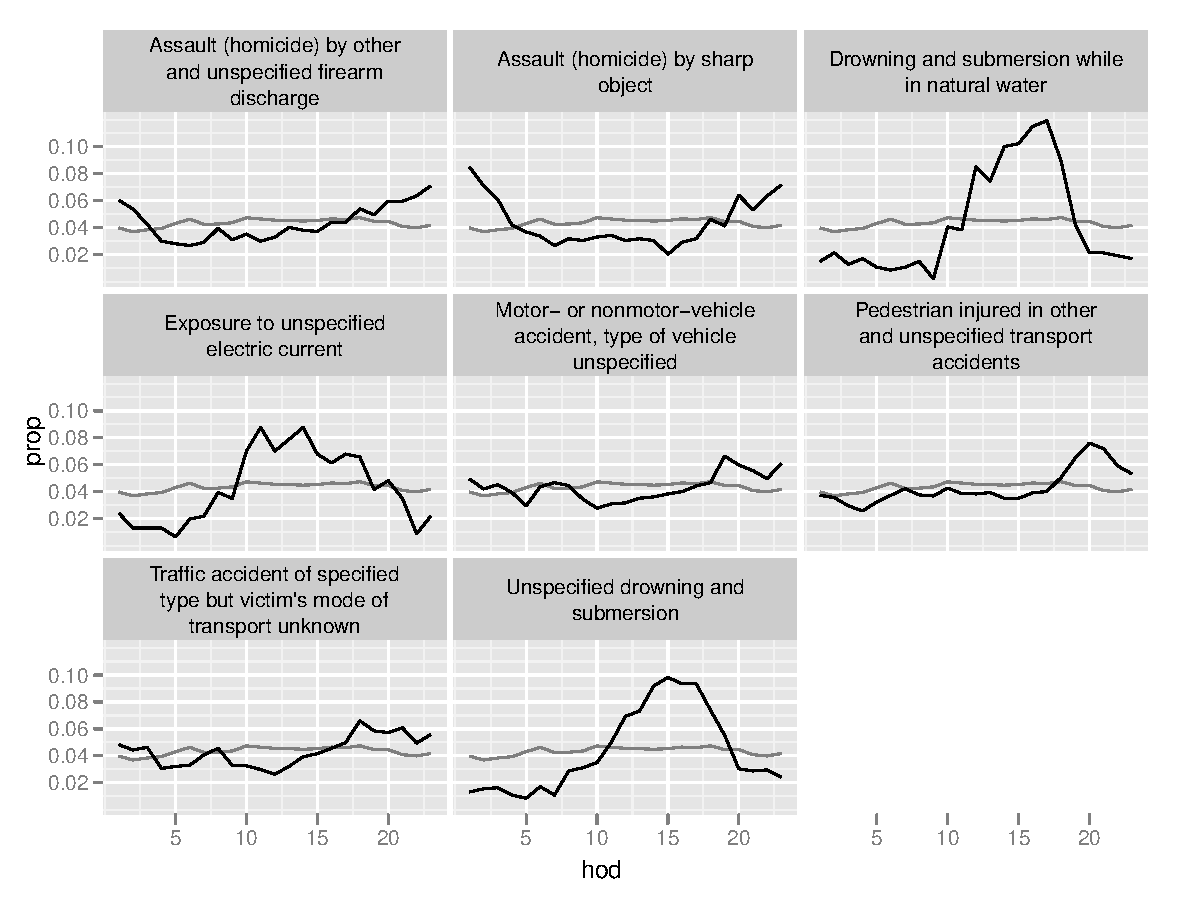
\includegraphics[width=0.9\textwidth]{case-study/unusual-big}
    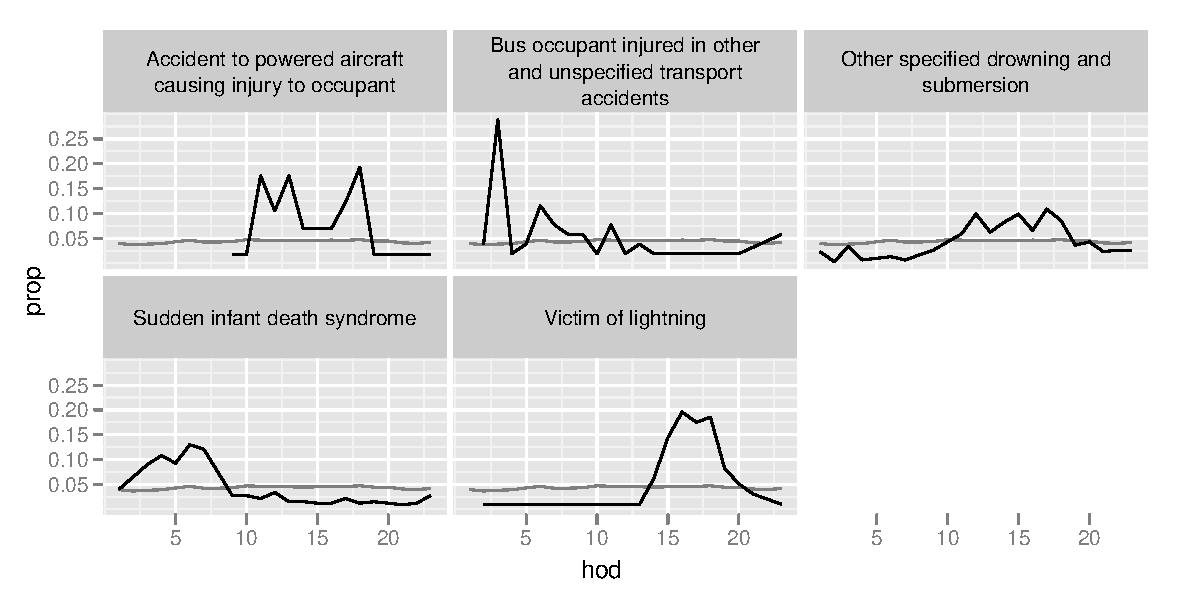
\includegraphics[width=0.9\textwidth]{case-study/unusual-sml}
  \caption{Causes of death with unusual time courses.  (Top) Causes of death with more than 350 deaths over a year.  (Bottom) Causes of death with less than 350 deaths.}
  \label{fig:disease}
\end{figure}

\begin{verbatim}
devi$resid <- resid(rlm(log(dist) ~ log(n), data = devi))
unusual <- subset(devi, resid > 1.5)
hod_unusual_big <- match_df(hod2, subset(unusual, n > 350))
hod_unusual_sml <- match_df(hod2, subset(unusual, n <= 350))
\end{verbatim}

\section{Conclusion}

% bibtool -x tidy-data.aux -c -o references.bib 
\bibliography{references}

\end{document}
